% Asset ID: AS1DifferentiationTIKZ-005
% Source: CCEA AS1-DIFF-LO008 + lesson sign-chart section
% Related lesson section: Core Theory 17
% Purpose: Show sign chart for f'(x)=3x^2-1 and increasing/decreasing intervals for f(x)=x^3-x.

\documentclass[tikz,border=8pt]{standalone}
\usepackage{amsmath}
\usetikzlibrary{arrows.meta}

\begin{document}
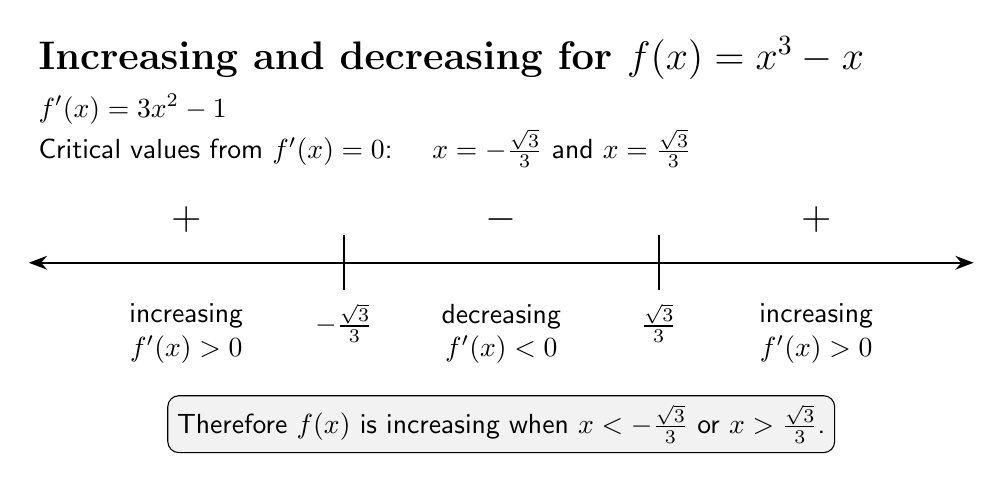
\begin{tikzpicture}[font=\sffamily, >=Stealth]

\node[anchor=west, font=\Large\bfseries] at (0,4.2) {Increasing and decreasing for $f(x)=x^3-x$};
\node[anchor=west] at (0,3.55) {$f'(x)=3x^2-1$};
\node[anchor=west] at (0,3.05) {Critical values from $f'(x)=0$: \quad $x=-\frac{\sqrt3}{3}$ and $x=\frac{\sqrt3}{3}$};

\draw[thick, <->] (0,1.6) -- (12,1.6);
\draw[thick] (4,1.25) -- (4,1.95);
\draw[thick] (8,1.25) -- (8,1.95);

\node[below] at (4,1.2) {$-\frac{\sqrt3}{3}$};
\node[below] at (8,1.2) {$\frac{\sqrt3}{3}$};

\node[font=\Large\bfseries] at (2,2.15) {$+$};
\node[font=\Large\bfseries] at (6,2.15) {$-$};
\node[font=\Large\bfseries] at (10,2.15) {$+$};

\node[align=center] at (2,0.7) {increasing\\$f'(x)>0$};
\node[align=center] at (6,0.7) {decreasing\\$f'(x)<0$};
\node[align=center] at (10,0.7) {increasing\\$f'(x)>0$};

\node[draw, rounded corners, fill=gray!10, align=center] at (6,-0.45)
{Therefore $f(x)$ is increasing when
$x<-\frac{\sqrt3}{3}$ or $x>\frac{\sqrt3}{3}$.};

\end{tikzpicture}
\end{document}
